\section{Guida utente}
La schermata iniziale del gioco presenta la scelta del numero di giocatori, e per ciascuno, dei campi in cui inserirne il nome e il relativo colore. Dopo aver selezionato e impostato a piacimento le informazioni dei giocatori, si dovrà semplicemente cliccare sul pulsante "Inizia una nuova partita". A questo punto si avrà accesso alla schermata di gioco, che si presenta come in figura.

\begin{figure}[ht]
    \centering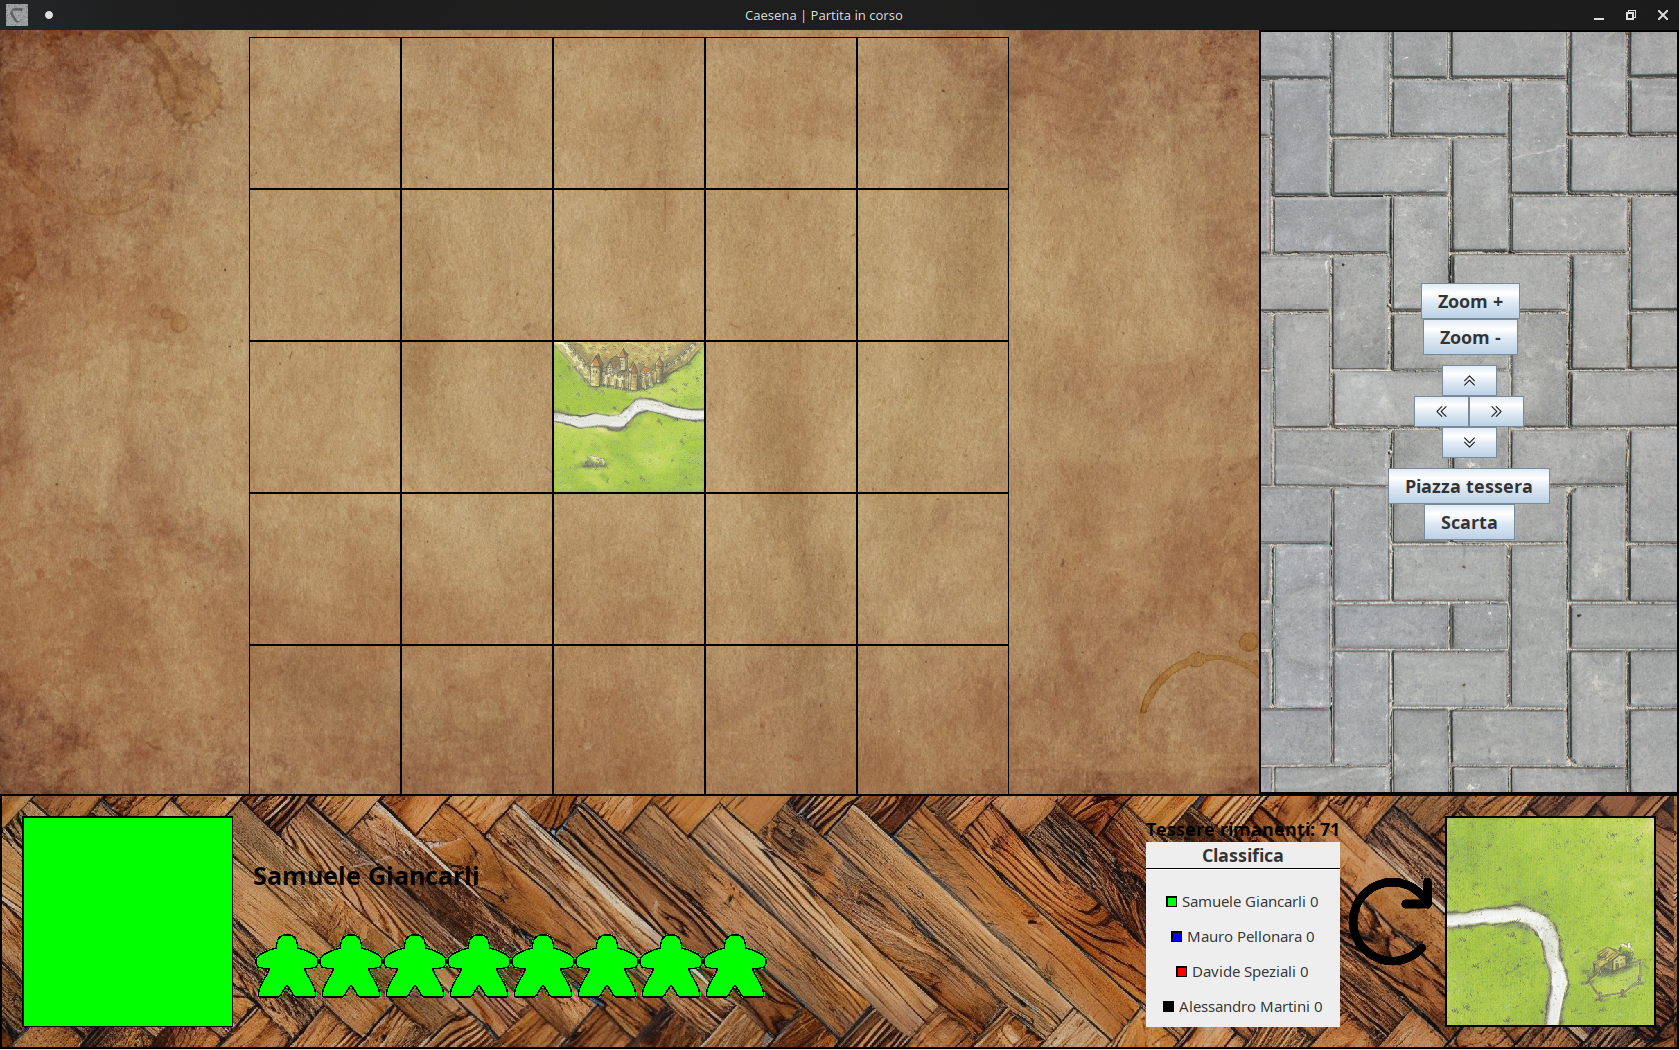
\includegraphics[scale=.25]{images/board.png}
    \caption{Schermata di gioco.}
\end{figure}

L'elemento principale del gioco è il tabellone che mostrerà al suo centro la tessera iniziale vicino alla quale dovranno essere piazzate le altre tessere. In basso a sinistra dello schermo vengono mostrati colore e nome del giocatore corrente oltre al numero dei suoi seguaci rimanenti, mentre alla destra si trovano la classifica dei giocatori e l'immagine della tessera corrente con il pulsante per ruotarla. A destra dello schermo si presentano invece i controlli del tabellone che ne gestiscono lo Zoom e ne permettono lo spostamento all'interno. Premendo il pulsante "Piazza tessera" questa verrà piazzata solo in caso sia stata selezionata una posizione nel tabellone. Premendo invece il pulsante "Scarta" verrà scartata la tessera solo se non piazzabile. Il pulsante "Piazza seguace" mostra invece l'apposita schermata che permette il piazzamento del seguace. Premendo "Finisci turno" si passa al turno successivo. Mentre si sta giocando è anche possibile aprire o chiudere il menù di pausa premendo ESC.
\medskip

Alla fine della partita, verrà mostrata la classifica finale nella quale ogni giocatore vedrà il proprio punteggio conclusivo e avrà la possibilità di tornare alla schermata iniziale o di uscire dal gioco.
\medskip

Il gioco supporta anche la lingua inglese nel caso il sistema operativo non utilizzi la lingua italiana, il testo dei pulsanti alla quale si riferisce la guida si traduce nel seguente modo:
\begin{itemize}
    \item "Inizia una nuova partita" $\rightarrow$ "Start a new game"
    \item "Piazza tessera" $\rightarrow$ "Place tile"
    \item "Scarta" $\rightarrow$ "Discard"
    \item "Piazza seguace" $\rightarrow$ "Place meeple"
    \item "Finisci turno" $\rightarrow$ "End turn"
\end{itemize}
